\documentclass{mpaper}
\usepackage{multirow}
\usepackage{subcaption}

\begin{document}

\title{Is Technical Debt Real?}
\author{Ovidiu Popoviciu}
\matricnum{2036725p}


\maketitle


\begin{abstract}
The concept of technical debt has received considerable attention in recent
years in both research and industry. Despite this, there is relatively little
empirical evidence as to the longer term impact of technical debt on a software
project. In our work, we seek to test the hypothesis that technical debt incurs
work-effort `interest' in a software project, arising through increased feature
implementation costs. In this paper, we test the correlation between technical
debt and work effort by measuring the cost of implementation of a work item
within five project histories and measuring the impact of technical debt on
implementation cost. It is hoped that this study is the first step in a series
on identifying technical debt and on provisioning of a decision-support method
to enable software project teams to make rationale long-term decisions as to the
management of quality issues. 
\end{abstract}

%%%%%%%%%%%%%%%%%%%%%%%%%%%%%%%%%%%%%%%%%%%%%%%%%%%%%%%%%%%%%%%%%%%%%%%%%%%%%%%
%%%%%%%%%%%%%%%%%%%%%%%%%%%%%%%%%%%%%%%%%%%%%%%%%%%%%%%%%%%%%%%%%%%%%%%%%%%%%%%
%%%%%%%%%%%%%%%%%%%%%%%%%%%%%%%%%%%%%%%%%%%%%%%%%%%%%%%%%%%%%%%%%%%%%%%%%%%%%%%
\section{Introduction}
\label{introduction}

% General description of the problem, motivation, relevance
The metaphor of technical debt was first proposed by \cite{Cunningham1993}, in
reference to the temporary sacrifice of code quality in exchange for the faster
delivery of features. Thus, incurring technical debt might be useful to achieve
immediate deadlines but may simultaneously have negative consequences for future
work, such as software complexity growth, the prevalence of bugs and defects,
decreased team productivity and augmented work effort, leading to increased
costs of development, infrastructure and management. The impact of technical
debt may affect the daily work of developers, project managers, product owners
and other stakeholders of the business.

Although initially intended as a metaphor, considerable research has since been
undertaken into the identification \cite{Lim2012}, measurement
\cite{Fontana2016} and management \cite{Codabux2013} of technical debt. Research
has also expanded the scope of the term, such that technical debt spans not just
activities related to code implementation but the entire software development
environment \cite{Power2013}. The research community identified multiple types
of debts \cite{Li2015}, each with its advantages and consequences if not handled
accordingly. Although industry practitioners are aware of its presence
\cite{Codabux2013} \cite{Lim2012}, there is no standard way of measuring the
current and future impact of technical debt on development and costs of the
team. Additionally, due to lack of vocabulary and complexities of the
phenomenon, developers find it difficult to convey their concerns to project
stakeholders \cite{Kruchten2012}.
 
For example, code smells and code violations are an example of technical debt
items that may increase future development effort and maintenance costs
\cite{Fowler1999}. Industry case studies have shown that such code violations
are more likely to be addressed if made visible by developers within the
project's issue tracker \cite{Lim2012}. However, from the perspective of a
project manager, it is essential to understand how much effort the team puts
into technical debt reduction activities and if there is an associated business
value. A key concern, therefore, is the ability to measure and make rationale
cost-benefit analyses of the impact of technical debt on productivity within a
project, capturing both the principal debt incurred and consequent interest, as
poor code quality accumulates.

% Research questions
The primary research objective of this work is to identify if there exists a
correlation between additional work effort caused by the presence of technical
debt in a code base through an empirical analysis of work effort in task
implementations within software projects. A further objective is to understand
how the measure of technical debt varies with software evolution and how do
specific development patterns are affected by debt. The research questions for
this study are as follows:

\begin{itemize}
	\item How does the cost of feature implementation vary with the magnitude of
	      technical debt?
	\item At what project `level' does technical debt affect developers most?
  \item How does work effort vary with the introduction of technical debt? 
  \item How does work effort vary with the removal of technical debt?
\end{itemize}

We adopted an empirical approach to the identification of the impact of
technical debt on the implementation of future features in existing software
code bases. To do this, we calculated the level of technical debt in the system
for each change-set recorded in a project's version control repository. We also
recorded the practical work effort spent on feature implementation by linking
data from a project's issue tracker and version control repository and thus
estimated the effort a developer spent on completing a work task. By
investigating these research questions, this study contributes:
\begin{itemize}
  \item A collection pipeline for acquiring and centralising data from three
  fundamental systems of any development environment;
  \item Two novel methods for computing work effort using data collected from
  five open source systems;
  \item A coherent method of calculating technical debt at the project and class
  level;
  \item A foundation for futher work in empirical analysis of technical debt and
  work effort.
\end{itemize}

% Section descriptions
Section \ref{background} mentions important state-of-the-art work that is will
build on, while section \ref{methodology} goes into data modelling, collection
and processing phases of the study. Finally, section \ref{results-discussion}
provide insights into results while section \ref{validity-future-work} states
the possible threaths to the validity of this experiment and further research
for expansion.

%%%%%%%%%%%%%%%%%%%%%%%%%%%%%%%%%%%%%%%%%%%%%%%%%%%%%%%%%%%%%%%%%%%%%%%%%%%%%%%
%%%%%%%%%%%%%%%%%%%%%%%%%%%%%%%%%%%%%%%%%%%%%%%%%%%%%%%%%%%%%%%%%%%%%%%%%%%%%%%
%%%%%%%%%%%%%%%%%%%%%%%%%%%%%%%%%%%%%%%%%%%%%%%%%%%%%%%%%%%%%%%%%%%%%%%%%%%%%%%
\section{Background}
\label{background}

There are many studies which have investigated the impact of technical
debt items on the costs of software projects. This section reviews this work
and relates the existing state of the art to our proposed experiment to
empirically measure the work effort interest accumulated by technical debt.

Olbrich et al. \cite{Olbrich2009} studied the impact of two code smells,
specifically God class and Shotgun Surgery, on change-proneness of class
entities and size of changes within two open source systems: Apache Lucene and
Apache Xerces. They found that classes containing smells are more change prone
than other, non-smelly, classes. In a similar study, Khomh et al.
\cite{Khomh2009} empirically analysed the impact of 29 code smells on the
change-sets of 9 releases of two open source systems. They had confirmed the
results of the previous studies that code smells increase the number of changes
that software undergoes during its evolution. Additionally, they had found that
classes containing more than one code smell are more subject to change more
often than others. 

Charalampidou et al. \cite{Charalampidou2017} introduced a study that assessed
the `interest probability' of code smells, which is the probability of a code
smell to introduce extra changes in future development. The authors calculated
the measurement by counting the frequency of each code smell and how it
correlated with the change-proneness of the module where it resides. They
studied smells such as Long Method, Conditional Complexity and Duplicated Code.
The results showed that code duplication had the highest interest probability,
due to the number of changes required to maintain future development. Moreover,
high cyclomatic method complexity increased the number of changes. Fontana et
al. \cite{Fontana2012} studied the impact of removing code smells on code
quality metrics such as cohesion, coupling and complexity. They applied
refactoring activities for each smell and re-evaluated the metrics. The results
showed that refactoring of one code smell might provide benefits for some code
qualities but may negatively impact others.

The authors studied the impact of code smells and their removal on the software
quality metrics output by directly analysing reports of code quality tools. In
comparison, our proposed work aims to focus on what impact quality issues and
bug patterns have on work effort costs by measuring technical debt at the
project and class levels. Additional studies have looked at quantifying
implementation cost in the context of technical debt.

Singh et al. \cite{Singh2014}, calculated interest payments by monitoring
development effort and code comprehension. They monitored time spent by
developers in classes with known debt items and implemented a tool within the
Integrated Development Environment of developers to gather information on class
visits and development session times. They quantified interest as the difference
between time practically spent in classes and an estimated, `ideal' time.
However, the study was conducted with the input of only one developer over a
period of 9 months. Additionally, estimating the most optimal time spent on
development is a challenging task due to numerous subjective factors such as
level of technical knowledge, familiarity with development environment and
personality traits.

Gomes et al. \cite{Gomes2011} studied the correlation between software
evolution, defect occurrence and work effort deviation at the release level. The
authors extracted data from documentation sources such as test plans, project
plan, weekly reports, project source code, and emails. Using this data, they
could derive important team information on change-sets, effort, quality, test
and size of the system. They measured extra work effort by subtracting the
estimated work time and total practical work time. Although information at the
release level offers project managers an idea of work effort deviation, it does
not show at a granular level what defects slow down development of a new feature
and where the team should focus their refactoring activities.

The initial study by Gomes et al. \cite{Gomes2011} provided a good start to
identifying work effort deviation. However, it only analysed major releases of a
system and did not provide drill-down information on iterations and code commits
on which features and code smells had the most effect on work effort. This is
essential information for developers and project managers to prioritise
refactoring activities in work iterations, especially in an Agile environment
where quickly responding to changes is a critical task
\footnote{http://agilemanifesto.org/}.

%%%%%%%%%%%%%%%%%%%%%%%%%%%%%%%%%%%%%%%%%%%%%%%%%%%%%%%%%%%%%%%%%%%%%%%%%%%%%%%
%%%%%%%%%%%%%%%%%%%%%%%%%%%%%%%%%%%%%%%%%%%%%%%%%%%%%%%%%%%%%%%%%%%%%%%%%%%%%%%
%%%%%%%%%%%%%%%%%%%%%%%%%%%%%%%%%%%%%%%%%%%%%%%%%%%%%%%%%%%%%%%%%%%%%%%%%%%%%%%
\section{Methodology}
\label{methodology}

In this paper, we present an approach for aggregating development team data
sources such as project management tools, version control logs and static
analysis results to produce a timeline of technical debt and work effort over
the evolution of a software product. Our motivation is to empirically find a
correlation between technical debt and the amount of work effort involved in
development of work items. In the absence of work tracking information,
aggregation of such data sources might provide a relatively accurate estimation
of the number of hours a developer has accomplished to complete a task.

When developing our approach, we completed the following steps:
\begin{enumerate}
  \item Designing an initial data model.
  \item Selecting data candidates (projects) that satisfy specific criteria.
  \item Collecting data from issue tracker, version control logs and generating
  static analysis output.
  \item Processing and refining data for analysis. 
\end{enumerate}

Section \ref{experimental-design} dives into the data model while section
\ref{data-selection} describes the data candidates criteria and selected
projects. The data collection process is described in Section
\ref{data-collection} while the calculation of work effort and technical debt is
described in Section \ref{data-processing}.

% - - - - - - - - - - - - - - - - - - - - - - - - - - - - - - - - - - - - - - -
\subsection{Experimental Design}
\label{experimental-design}

The initial step was to design a model of the aggregated data and to understand
what type of information each selected data source will provide. We consider the
following fundamental data sources of any development environment relevant to
the collection of data:

\begin{itemize}
  \item A \emph{Version Control System} is a system that manages changes to the
  source code. As work items are implemented, the system logs all changes made
  by the development team. The most popular version control tool is Git
  \footnote{https://git-scm.com/}.

  \item \emph{Project Management Tools} are software systems that help teams
  track, manage and collaborate on various types of units of work. A common
  example of a complex project management tool is Jira
  \footnote{https://www.atlassian.com/software/jira}. GitHub
  \footnote{https://github.com/} and BitBucket
  \footnote{https://bitbucket.org/}, which are code hosting platforms, also
  provide an issue tracking tool with each code repository.
  
  \item \emph{Static Analysis Tools} analyse the source code for quality issues,
  security flaws and adherence to industry standards.There are many examples of
  static analysis tools: Spotbugs \footnote{https://spotbugs.github.io/}
  (formerly FindBugs), SonarQube, CAST, Sonargraph.

\end{itemize}

All the data sources contain detailed information related to project
requirements and small tasks, to the set of changes that the source code has
suffered over time and to the possible quality issues the development team might
encounter. In many cases, development teams use various systems from different
vendors with little or no `common ground' between them. They are considered
separate services that run in isolation to one another. The data collection
pipeline must have features to interact with each service. Fortunately, forms of
integration exists between these services for productivity purposes. An example
is linking work items to change-sets by specifying the work item ID in the a
revision title. This integration provides valuable guidance on how many
revisions the source code has suffered during the implementation of a work item.

The centralised data model, presented in Figure \emph{FIGURE}, highlights the
integration of version control logs, issue tracker data and static analysis
output. The next few sections highlight the information collected from each data
source.

% - - - - - - - - - - - - - - - - - - - - - - - - - - - - - - - - - - - - - - -
\subsubsection*{Version Control}
\label{version-control}

The version control system keeps track of the evolution of source code over
time. It tracks and logs changes deployed by developers on a daily basis. Such
logs are indispensable, since the metadata associated with them provides direct
information on implementation patterns of the development team.

As mentioned, Git is a simple version control tool that tracks changes of the
source code using branching model. Each repository contains at least one
development line, called a ``branch''. The main development branch is commonly
named the \emph{master} branch. Branches contain a stream of small units of
work, called ``commits'', which are the snapshots of the source code at a
particular point in time. Additionally, each commit contains relevant metadata
with the following fields:

\begin{itemize}
  \item \emph{Object ID} - is the identifier of the snapshot;
  \item \emph{Author} - the name (or username) of the person who originally
  wrote the change;
  \item \emph{Message} - a short description of the change-set;
  \item \emph{Timestamp} - the time when the commit was created;
  \item \emph{Diff} - the set of changes that the source code has suffered, when
  compared to the previous commit. 
\end{itemize}

Teams can `integrate' their version control system with an issue tracker such
that changes can be directly linked to the appropriate ticket. The most common
method is to specify the ticket ID in the message of the commit. As a result, it
is simpler to find out which change-sets belong to a particular work item. 

For a project managed using Git, all the metadata fields can be retrieved from a
clone of the repository on a local computer. This makes Git a powerful tool in
studying the history of changes and evolution of any software product.

% - - - - - - - - - - - - - - - - - - - - - - - - - - - - - - - - - - - - - - -
\subsubsection*{Project Management}
\label{project-management}

Project management tools allows developers and project managers to keep track of
the work that must be accomplished and of the issues that have been reported by
the users of the software. 

Each work item is represented in the form of a \emph{ticket}, which is a report
of the work that needs to be completed. Depending on the workflow of the team,
tickets may go through various `transitions', which are changes to the ticket
made by a team member. For example, changes to the `status` field of a ticket
represents a transition from one status to another. A ticket may contain many
relevant metadata fields, including:

\begin{itemize}
  \item \emph{ID} - the unique identifier of the work item in the project;
  \item \emph{Type} - the type of work e.g. Task, Feature, Bug or Enhacement;
  \item \emph{Status} - the current status of the work e.g. Created, In
  Progress, Testing, In Review, Closed;
  \item \emph{Summary} - a brief description of the task;
  \item \emph{Description} - a longer, more detailed description;
  \item \emph{Priority} - the importance of the work as considered by the team;
  \item \emph{Assignee} - the team member responsible for completing the work;
  \item \emph{Story Points} - an estimation or measurement of complexity;
  \item \emph{Comments} - a list of comments by other team members to promote
  discussion;
  \item \emph{Timestamps} - the times when ticket was created, updated, closed
  and what point it is due.
\end{itemize}

Moreover, Jira tickets contain a field called \emph{Time Tracking} that
allows tracking of the estimated time to complete the work, time logged and time
left. Moreover, for Jira, the history of changes of a work item is available
through its API in a field called \emph{Transitions}. This field may provide
valuable information of development patterns, by analysing the changes of the
status field over ticket lifetime. 

Although project management tools provide relevant work tracking information,
not all offer the same broad scope of work data. For example, the integrated
issue tracker within GitHub and BitBucket do not offer the same features and
functionality that Jira does. Additionally, many of the fields of tickets might
be non-existent which poses a problem when computing a measure of work effort.

% - - - - - - - - - - - - - - - - - - - - - - - - - - - - - - - - - - - - - - -
\subsubsection*{Static Analysis}
\label{static-analysis}

% intro
Static analysis tools provide an elegant method of analysing source code for
possible weaknesses and quality issues without a direct execution of the entire
product. Its applicability makes it an excellent tool for developers to analyse
their change-sets at any time of the implementation process.

% body
Although static analysis tools provide an approximate measure of the quality of
the code base, there is a danger in associating technical debt with their
output. There are multiple types of technical debt present in the software
development environment \cite{Li2015}. For example, static analysis tools cannot
predict that the requirements gathering phase was not completed appropriately
and thus it might take more time for a team member to understand the
expectations of a work item and indirectly increasing effort required to
complete the task. In this study, we consider that only code debt affects the
work effort for completing a task, as a simplifying assumption to aid in the
calculation of work effort. 

The output of static analysis tools are, generally, weaknesses and bugs that may
lead to vulnerabilities of the product. We consider such code violations as the
`lowest level' of technical debt, named code debt, which is the technical debt
that developers encounter daily \emph{Avgeriou2016}. There are many static
analysis tools, many of which have been reviewed by current research
\cite{Fontana2011}. 

In general, the output of a code analysis tool, including SpotBugs, contains:
\begin{itemize}
  \item \emph{ID} - a unique identifier of the quality issue;
  \item \emph{Severity} - a measure of severeness e.g. High, Medium, Low;
  \item \emph{Description} - a short description of the code violation;
  \item \emph{Location} - the location of the quality issue, represented by the
  file name and line number. 
\end{itemize}

This type of output gives a representation of the possible low-level weaknesses
that developers might introduce and encounter during the implementation process.
Additionally, by using the version control logs it is possible to track the
items that have been introduced or removed for each change-set as well as the
total amount of issues that an author dealt with. 

Unfortunately, not all projects use a static analysis tool to check for issues
and, if some do, the historical technical debt for each possible revision is
non-existent. For this reason, in the data collection process, we are using a
single static analysis tool to review historical debt items for each project.

% - - - - - - - - - - - - - - - - - - - - - - - - - - - - - - - - - - - - - - -
% - - - - - - - - - - - - - - - - - - - - - - - - - - - - - - - - - - - - - - -
% - - - - - - - - - - - - - - - - - - - - - - - - - - - - - - - - - - - - - - -
\subsection{Candidates selection}
\label{data-selection}

% intro
We applied the data collection and processing stages to a set of real,
open-source software projects. Initially, from a choice of 11 open-source
libraries and development tools, we have selected the following candidates: 

\begin{itemize}
	\item ANTLR \footnote{https://github.com/antlr/antlr4} - ``s a powerful parser
	      generator for reading, processing, executing, or translating structured text
	      or binary files'';
	\item Spring HATEOAS
	      \footnote{https://github.com/spring-projects/spring-hateoas} - ``Library to
	      support implementing representations for hyper-text driven REST web services
	      ''
	\item Checkstyle \footnote{https://github.com/checkstyle/checkstyle} - ``is a
	      development tool to help programmers write Java code that adheres to a coding
	      standard'';
	\item Apache Commons Collections
	      \footnote{https://github.com/apache/commons-collections} - ``contains types
	      that extend and augment the Java Collections Framework'';
	\item Apache Commons Lang \footnote{https://github.com/apache/commons-lang} -
	      ``a package of Java utility classes for the classes that are in java.lang's
	      hierarchy, or are considered to be so standard as to justify existence in
	      java.lang''.
\end{itemize}

To be included in the study, a project must satisfy a list of rigorous criteria:

\begin{itemize}
  \item Use Git as a version control tool. due to its powerful features,
  applicability and popularity. Additionally, the project must be open-source to
  access the history of snapshots.
  \item Use a project management tool that is publicly accessible to retrieve
  work item data.
  \item Use Java \footnote{https://java.com/en/} as the main programming
  language. This was a simplifying criteria to keep the data collection and
  processing consistent.
  \item The project should have a single main development branch, preferably the
  ``master'' branch. This relieves the data collection process of analysing
  multiple branches.
  \item The version control hosting system should integrate with the project
  management tool to highlight the commits that belong to a specific work item.
  \item The project uses Maven \footnote{https://maven.apache.org/} as its build
  system due to simplifications in development process of the data collection
  tool.
\end{itemize}

\begin{table}
	\begin{tabular}{|l|r|c|}
    \hline
		\emph{Project Name}        & \emph{Size (LOC)} & \emph{Issue Tracker}  \\ \hline \hline
		ANTLR                      & 399,388            & GitHub               \\ \hline
		Spring HATEOAS             & 25,601             & GitHub               \\ \hline
		Checkstyle                 & 353,273            & GitHub               \\ \hline
		Apache Commons Collections & 124,854            & Jira                 \\ \hline
		Apache Commons Lang        & 158,713            & Jira                 \\ \hline
	\end{tabular}
	\caption{\label{tab-data-candidates} Data candidates}
\end{table}

% body 
Table \ref{tab-data-candidates} shows the selected open-source projects that
have their data collected and analysed as well as their size (LOC), version
control and project management tools. Out of the initial project pool, we have
only included five for analysis of results due to an incomplete data collection
process, as a result of:

\begin{itemize}
  \item Unavailable APIs for accessing project management tool.
  \item Non-existent historical static analysis results. This might be due to a
  ``Zero Bugs'' policy set by the development team 
  \item Failing build process for the majority of revisions. The build process
  was failing on too many revisions and thus the static analysis stage could not
  be completed.
\end{itemize}

% - - - - - - - - - - - - - - - - - - - - - - - - - - - - - - - - - - - - - - -
% - - - - - - - - - - - - - - - - - - - - - - - - - - - - - - - - - - - - - - -
% - - - - - - - - - - - - - - - - - - - - - - - - - - - - - - - - - - - - - - -
\subsection{Data collection}
\label{data-collection}

% intro
To collect relevant data for each candidate project, we designed and implemented
a tool that collects data from version control logs, project management tools
and statically analyses the source code on each revision. The result are
collected into a single, centralised database for further processing and
analysis. The tool has been built using Java and open-source technologies, and
is publicly available \footnote{https://github.com/ovidiup13/tdanalysis}. It
relies on the following dependencies:

\begin{itemize}
  \item jGit \footnote{https://www.eclipse.org/jgit/} - is a Java library for
  interacting with the Git version control system;
  \item REST Java Client for Jira
  \footnote{https://bitbucket.org/atlassian/jira-rest-java-client} - is a Java
  library that provides a simple interaction with Jira APIs;
  \item GitHub API for Java \footnote{http://github-api.kohsuke.org/} - is a
  Java library that provides integration with GitHub API for retrieving issues;
  \item MongoDB \footnote{https://www.mongodb.com/} - NoSQL database technology
  for storing collected data;
  \item Spotbugs - tool for identifying bug patterns in source code.
\end{itemize}

The data collection process is shown in figure \emph{FIGURE}. Firstly, each
candidate project repository is cloned to local storage. Secondly, the tool
starts the `collection step', where each revision of the project history is
processed serially, starting with the latest revision and going back in time.
The collection step is composed of multiple sub-steps:
\begin{enumerate}
  \item \emph{Retrieve commit metadata}. Interacts with Git to retrieve relevant
  data from each revision;
  \item \emph{Search and retrieve ticket(s)}. The current commit message is
  analysed for mentions of ticket IDs. For any ticket ID found, the tool
  retrieves the ticket from the project management tool API;
  \item \emph{Build current revision}. This is a preparation step for the static
  analysis. The source code of the project must be compiled into classes and
  packaged into JARs for static analysis to complete;
  \item \emph{Analyse JARs}. Scan the current revision for quality issues. If
  the build process fails, then the static analysis scan is skipped, due to
  missing JAR files. 
\end{enumerate}

Data is stored at the end of each substep to avoid an inconsistent commit stream
in case one of the next one fails or the tool crashes. Additionally, this method
allows us to reproduce the experiment without any outside changes to the dataset
while future work items do not incur an additional data collection overhead.
Moreover, due to the choice of a NoSQL database technology, we can introduce new
data points from additional projects without any breaking changes to the initial
data model. 

During development, the building and static analysis steps incurred an extreme
overhead that was slowing down the data collection process. For a repository
with thousands of revisions, the build and analysis steps incurred a significant
time overhead that would overstep the timeline of the experiment. Therefore, the
build process was customised by skipping a few unnecessary tasks that we did not
consider in scope for this experiment such as generating documentation,
compilation and running of tests and test coverage analysis. Another key point
is that some projects were running custom static analysis step as part of the
build process. We decided to skip it due the decision to run Spotbugs analysis
and to optimise the current process. 

Additionally, the tasks that compile and run the testing suites were ignored.
Firstly, testing was considered a separate activity to the implementation of new
features, fixing bugs and adding enhacements. Thus, in this case, code debt was
split into `code debt' and `testing debt'. Testing debt refers to shortcuts
taken during the testing phases. Secondly, the testing task added an additional
overhead to the build process. However, in reality, testing is a fundamental
part of development and is tightly integrated with implementation of work items,
especially in the practice of Test Driven Development. It is one of the top most
mentioned types of technical debt in a mapping study by Li et. al \emph{Li2015},
along with code, architecture and design debt. The integration of testing debt
within this experiment is considered as a future work item, mentioned in section
\ref{future-work}.

\begin{table*}[t]
	\centering
	\begin{tabular}{|l|r|r|r|r|r|}
		\hline
		Category                & \emph{ANTLR} & \emph{Spring HATEOAS} & \emph{Checkstyle} & \emph{Commons Collections} & \emph{Commons Lang} \\ \hline \hline
		Total Commits           & 728          & 539                   & 1,814             & 3,306                      & 5,061               \\ \hline
		Total Tickets           & 215          & 173                   & 188               & 236                        & 304                 \\ \hline
		Build Successful        & 478          & 472                   & 1,732             & 392                        & 3,814               \\ \hline
		Build Failed            & 250          & 67                    & 82                & 2,914                      & 1,247               \\ \hline
		Commits with Tickets    & 217          & 327                   & 1,157             & 437                        & 1,306               \\ \hline
		Commits without Tickets & 511          & 212                   & 657               & 2,869                      & 3,755               \\ \hline
		Ticket / Commit         & 0.217        & 0.744                 & 0.654             & 0.034                      & 0.258               \\ \hline
	\end{tabular}
	\caption{\label{tab-data-collection} Data collection results}
\end{table*}


% conclusion
The results of the data collection process are shown in Table
\ref{tab-data-collection}. Although only 5 projects have been selected out of
the initial pool, we have managed to retrieve and analyse approximately
\emph{10,000} commits and \emph{1,000} work items along with an average of over
\emph{100} unique quality issues. Section \ref{results-discussion} dives into
the results of our analysis. 

% - - - - - - - - - - - - - - - - - - - - - - - - - - - - - - - - - - - - - - -
\subsection{Data processing}
\label{data-processing}

% intro
The collection step gathered data from three systems and stored them into a
single source of truth for further processing. Therefore, this stage was
implemented in the tool to allow the calculation of work effort and technical
debt, at various `levels' of the project. Additionally, the tool allows the
results to be displayed and analysed visually.

% body
The processing stage revolved around the concept of \emph{work items}. A work
item is a specific tasks assigned to a developer and each item is composed of a
ticket and a list of revisions, ordered chronologically. A ticket is the report
of the work, which represents the data retrieved from the project management
tool. the pieces of data retrieved from the project management tool. Similarly,
the list of revisions represent a subset of the total commits from the version
control system are linked to the specific ticket. As mentioned in section
\ref{data-collection}, commits are assumed to belong to a specific ticket if
their commit message references the ticket ID of the project management tool.

For each work item, we compute the following measures:
\begin{itemize}
  \item Work effort ($WE_{w}$) - the total number of hours a team member has
  exhausted to complete task $w$;
  \item Technical Debt ($TD_{w}$) - the total number of technical debt items
  that have affected the work, during implementation of task $w$.
\end{itemize}

We describe the methods of calculation for each measurement separately, in the
following sections. 

% - - - - - - - - - - - - - - - - - - - - - - - - - - - - - - - - - - - - - - -
\subsubsection*{Work Effort}
\label{work-effort}

% calculation of work effort
The work effort represents the total number of hours accomplished a single
developer towards the implementation of a work item $w$. Ideally, the project
manager would require developers to track the time spent on each task to
possibly help with future estimation of work effort for similar items.
Unfortunately, the majority of projects do not track such data and thus we have
designed calculations to estimate it from various systems of the development
environment.

To start, we considered that an item of work followed a linear pattern and that
a team member was working on a single work item at a time. Each $w$ has a start
time $t_{start}$ and end time $t_{end}$, both expressed as timestamps in
Greenwich Mean Time (GMT) format. A simple method for calculating $WE_{w}$ is to
take the difference between these two timestamps. This makes it easy to
calculate the working hours on the same day:

\begin{equation}
  \label{eq-work-effort-simple}
  WE_{w} = hours(t_{end} - t_{start})
\end{equation}

For example, if a developer starts work on $w$ on Monday at 9:00 GMT and
finishes work at 15:00 GMT, then the total of effort put in is 6 hours. However,
a work item might span multiple days and thus it would include time outside the
normal working hours. To cover for this case, we introduced another simplyfing
assumption. We assume that the normal working hours per day would not exceed 8
hours and this allows normalisation of hours according to the number of days
between the start and end times. This means that work spread over multiple days
would be calculated as follows:

\begin{equation}
  \label{eq-work-effort-days}
  WE_{w} = 8 * (days(t_{end} - t_{start}) + 1)
\end{equation}

If $w$ spans multiple days, then the total effort is the total number of
days multiplied by the number of working hours per day. For example, let's
assume that a developer starts a work item on Monday, 9:00 GMT and finishes his
work on Tuesday, 21:00 GMT. This equation will yield 16 hours of work spanning
two days (Monday and Tuesday). We recognize that there are multiple factors that
affect the work effort put in for a work item which are not modelled as part of
the calculation. For example, this equation does not exclude weekends or other
possible time off periods. 

From the data available, there are two sets of timestamps that could be used for
work effort calculation: \emph{commit timestamps} and \emph{ticket timestamps}.
Metadata of the project management tool might provide an accurate estimation of
the times an engineer has started and finished his work, provided that the team
follows a regulated workflow for transitioning tickets. Additionally, version
control logs provide additional metadata of each commit, including the time
where a commit was pushed to the repository. 

% a. by ticket
The ticket is a running `report' of the work involved. In the issue tracker, it
represents a reference point for the project manager, other members of the team
and for the assignee. As mentioned in section \ref{experimental-design}, the
ticket contains various fields and metadata, out of which the most of relevant
for calculating work effort are:

\begin{itemize}
  \item `Created' timestamp - the timestamp when the ticket was created and
  added to the project management tool;
  \item `Closed' timestamp - the timestamp when the ticket was marked as
  resolved or closed.  
\end{itemize}

The difference between these two timestamps might give an accurate estimation of
the number of hours, calculated using equations \ref{eq-work-effort-simple} and
\ref{eq-work-effort-days} mentioned above. However, they might not reflect the
implementation time accurately. For example, there might be an additional time
period between when a ticket was added to the issue tracker and when it got
picked up for development. For example, a ticket may have been created for a
week before the start of a new sprint, should the team employ an agile
development methodology. Moreover, if the team employs code review practices for
each piece of work, the closing date of the ticket might be after the work has
been reviewed by the rest of the team. Overhead time is problematic, as the
calculations may not be accurate. 

Fortunately, Jira contains an additional metadata field, called
\emph{Transitions} that lists the history of changes that the ticket has
suffered. Status changes are changes in the workflow of the ticket, such as from
\emph{Open} to \emph{In Progress} and from \emph{In Progress} to \emph{In
Review}. The timestamps of these transitions give a more accurate time range of
development work hours. GitHub and BitBucket do not have the transition feature
build-in.

As a result, the choice of timestamps for $t_{start}$ and $t_{end}$ based on
ticket metadata are as follows:
\begin{equation}
  \label{eq-ticket-start}
  \begin{aligned}
    t_{start} = Timestamp(Transition(\textrm{Open to In Progress})) \\ 
      \textrm{or} \quad Timestamp(\textrm{Created})
  \end{aligned}
\end{equation}

\begin{equation}
  \label{eq-ticket-closed}
  \begin{aligned}
    t_{end} = Timestamp(Transition(\textrm{In Progress to Closed})) \\ 
      \textrm{or} \quad Timestamp(\textrm{Closed})    
  \end{aligned}
\end{equation}

% b. by commit
An alternative set of timestamps may be used from version control logs. The
timestamp of a revision flags the date and time when a set of changes have been
applied. Since a work item may be composed of multiple revisions, a relatively
accurate estimation of work effort can be derived. 

To define the equation formally, we consider $C$ as the total list of commits of
the project and $w$ as a work item. For each work item $w$, $C_{w}$ is the
subset of $C$ of all commits that belong to the work item $w$. Commits for each
work item are labelled as $C_{w}[i]$ where $i$ is the commit position in $C[w]$,
$i=1...,n$ and $n$ is the number of commits associated with work item $w$.
Commits are ordered chronologically, in the order of development.

Therefore, to get a simple estimation of work effort we take the time difference
between the last commit $C_{w}[n]$ and first commit $C_{w}[1]$. Using this
method, $t_{end}$ accurately reflects the time of the last changes pushed by a
developer, which is the timestamp of $C_{w}[n]$, while $t_{start}$ represents
the timestamp of $C_{w}[1]$. However, the first commit $C_{w}[1]$, represents
the time when the changes have \emph{already} been implemented. In this case,
there is a margin of error introduced and the results are short of the
initial effort accomplished before the first commit has been finalised.

To cover for this case, we assume that once a contributor finished a work item
$w$ she would directly get started on $w+1$. If we are calculating the work
effort for work item $w$, we consider that the missing work effort is measured
as the number of hours between the last commit timestamp of the previous work
item $C_{w-1}[m]$ and the last commit timestamp $C_{w}[n]$ of the current work
item. As a result, we can consider commits as a continuous stream of work
changes, where one change follows the next in line. However, a developer may not
have a previous contribution to the project. In this case, the number of hours
simply cannot calculated accurately. Thus, the first commit $C_{w}[1]$ time of
the current work item is used as a starting point.

The selected timestamps for commits are chosen as follows:
\begin{equation}
  \label{eq-commit-start}
  \begin{aligned}
    t_{start} = Timestamp(C[w-1]_{m}) \quad or \quad Timestamp(C[w]_{1})
  \end{aligned}
\end{equation}

\begin{equation}
  \label{eq-commit-end}
  \begin{aligned}
    t_{end} = Timestamp(C[w]_{n})
  \end{aligned}
\end{equation}

Measuring work effort accurately from limited data is a challenging task. Most
open-source projects rely on contributions from software professionals all over
the globe. In an ideal case, developers would measure their work time on the
project management tool or on an internal worksheet. However, 54\% of software
professionals working remotely do not track their work effort
\cite{DeveloperSurvey2018}. As a result, we have considered two novel ways of
computing an estimate of work effort from project management tools and version
control logs. Although the two methods are not perfectly accurate, they provide
a good initial measurement of development times. The drawbacks are discussed in
section \ref{validity-future-work}.

% - - - - - - - - - - - - - - - - - - - - - - - - - - - - - - - - - - - - - - -
\subsubsection*{Technical Debt}

% calculation of technical debt
As mentioned in section \ref{background}, many state-of-the-art calculations for
technical debt have been implemented \cite{Letouzey2012} \cite{Nugroho2011}
\cite{Fontana2016}. The measure depicting the cost of paying back the debt at
the present time is often called the \emph{principal} while the extra cost of
development when keeping hold of items is called \emph{interest}. Unfortunately,
there is no standardised method of calculating a global technical debt index,
due to difficulties managing complexities of quantifying work effort and
development costs. Moreover, there is no single best tool for this purpose, as
all take into consideration various variables for metric computation. 

% total
We calculate the total technical debt $TDT_{w}$ for a work item $w$ at by simply
counting the total quality issues found by the static analysis tool at the start
of $w$. The start of $w$ is the reference point given by commit $C_{w}[1]$.
However, as mentioned before, the first commit already represents work completed
for $w$, not the work at the start of the item. Thus, we refer to the last
commit of the previous work item $w-1$ that was implemented \emph{before}
$C[w]_{1}$. Therefore, the `total pain' for $w$, at the project level, is given
by the total debt of the last revision of $w-1$, namely $TDT_{w-1}[m]$. Figure
\emph{FIGURE} shows a visualisation of the total technical debt of a work item.

% added, removed, remaining
Furthermore, we calculate the technical debt introduced and removed per work
item. The calculations are straightforward. The technical debt introduced
$TDI_{w}$ for a work item $w$ is the set difference between all technical debt
items in $C_{w}[n]$ and $C_{w-1}[m]$. That is, the technical debt introduced
represents all items which are in $TD_{w}[n]$ and are not in $TD_{w-1}[m]$, and
$TD_{w}[i]$ represents the set of technical debt items in work item $w$,
revision $i$.

\begin{equation}
  \label{eq-td-introduced}
  \begin{aligned}
    TDI_{w} = TD_{w}[n]  \setminus TD_{w-1}[m]
  \end{aligned}
\end{equation}

Similarly, the technical debt removed is the same set difference, inversed. That
is, the difference is  The remaining technical debt, is the total number of
technical debt items that have remained untouched during the feature
implementation. Figure \emph{FIGURE} shows a Venn diagram of the introduced,
removed and remaining technical debt per work item. 

\begin{equation}
	\label{eq-td-introduced}
	\begin{aligned}
		TDR_{w} = TD_{w-1}[m]  \setminus TD_{w}[n]
	\end{aligned}
\end{equation}

% locality
Although, we measured technical debt at the project level, the effort put in for
a work item may not be affected by all quality issues found in the \emph{entire}
project. For example, a trivial work item might include only a few small changes
to classes or configuration files. Therefore, the total pain of a work item may
depend on the total number of changes that a team member has implemented. We
consider that the technical debt items that have the most impact on work effort
are `local' to the change-set.

To calculate the local technical debt $TDL_{w}$, we calculate the total
change-set $CS_{w}$ per work item $w$. The total number of change-sets over a
work item is the total number of distinct files that have been added, removed or
modified during the implementation:

\begin{equation}
  \label{eq-td-changes}
  \begin{aligned}
    CS_{w} = CS_{w}[1] \cup CS_{w}[2] \cup ... \cup CS_{w}[n]
  \end{aligned}
\end{equation}

To find $TDL_{w}$, we intersect the set of technical debt items $TD_{w}$ with
the total change-sets:

\begin{equation}
  \label{eq-td-local}
  \begin{aligned}
    TDL_{w} = TD_{w} \cap CS_{w}
  \end{aligned}
\end{equation}

Hence, to find the technical debt items that might have an effect on work effort
locally, we find all classes that contain those items and intersect them with
the classes that have been changed during the revision. In this way, we get a
sense of potential quality issues that might affect development effort. Figure
\emph{FIGURE} shows a Venn diagram of the two sets and their intersection, which
signifies the total technical debt items local to the work item.\\

% conclusion
The processing stage was implemented as a request-reply server, running a REST
API \footnote{https://github.com/ovidiup13/tdanalysis}. Each request contains a
repository ID to identify the database entries, and the server calculates the
work effort and technical debt as required, for each project in isolation. The
calculation becomes computationally expensive as the size of the repository data
grows (number of issues and commits). Appropriate caching optimisations have
been implemented to minimise computation and speed up retrieval of results.
Moreover, we designed a Single Page Application (SPA) dashboard
\footnote{https://github.com/ovidiup13/tdanalysis-dashboard/} that connects to
the web server and displays statistics and charts for each project.


%%%%%%%%%%%%%%%%%%%%%%%%%%%%%%%%%%%%%%%%%%%%%%%%%%%%%%%%%%%%%%%%%%%%%%%%%%%%%%%
%%%%%%%%%%%%%%%%%%%%%%%%%%%%%%%%%%%%%%%%%%%%%%%%%%%%%%%%%%%%%%%%%%%%%%%%%%%%%%%
%%%%%%%%%%%%%%%%%%%%%%%%%%%%%%%%%%%%%%%%%%%%%%%%%%%%%%%%%%%%%%%%%%%%%%%%%%%%%%%
\section{Experimental evaluation}
\label{evaluation}

To explore the results of the data processing phase, we have conducted the
following experiments:

\begin{enumerate}
  
  \item Firstly, it is necessary to understand whether technical debt and work
  effort are correlated. This experiment was split in two parts respective of
  the two methods of computing work effort: using ticket and commit timestamps.
  Technical debt was computed simply as a count of all technical debt items at
  the project level. The aim was to understand whether work effort is impacted
  by a global technical debt measurement. We assumed that the type and work item
  complexity are constant.

  \item Secondly, to determine how debt items impact work directly at the code
  level, we experimented with the locality calculation model. We computed the
  local technical debt for each work item and compared that to the initial
  calculation of work effort. The purpose was to verify whether work effort was
  negatively impacted by technical debt at the local level. 
  
  \item Thirdly, we wanted to see if patterns of development affect task
  productivity. More specifically, the aim is to understand if introducing
  technical debt would speed up development time (reduce work effort) and if
  removing technical debt, as a potential refactoring activity, would increase
  development time (increase work effort).
\end{enumerate}

The experiments have been conducted incrementally, one after the other, in
parallel with development on the data processing stage.  

% - - - - - - - - - - - - - - - - - - - - - - - - - - - - - - - - - - - - - - -
\subsection{Results and Discussion}
\label{results-discussion}

For each repository, we calculated the mean and standard deviation to get a
sense of what the computed effort (in hours) is per work task. The comparison
between work effort calculations could be considered an experiment by itself.
However, since there is no way to evaluate the results without interacting
directly with collaborators of the project, we analysed the results by computing
the mean and standard deviation of all data points. Although the data analysis
techniques present are trivial, they provide a good overview of the distribution
of work effort over all work items in the project. The results of the work
effort calculation can be seen in table \ref{tab-work-effort}.  

\begin{table*}[t]
	\centering
	\begin{tabular}{ |c|c|r|r|r|r|r| }
		\hline
		\multicolumn{2}{ |c| }{Type}                     & \emph{ANTLR} & \emph{Spring HATEOAS} & \emph{Checkstyle} & \emph{Commons Collections} & \emph{Commons Lang} \\ \hline \hline

		\multicolumn{1}{ |c  }{\multirow{2}{*}{Ticket} } &
		\multicolumn{1}{ |l| }{Mean (hours)}             & 274.068      & 659.071               & 596.268           & 10,043.91                  & 2,918.43            \\ \cline{2-7}
		\multicolumn{1}{ |c  }{}                         &
		\multicolumn{1}{ |l| }{Std (hours)}              & 827.071      & 1,719.20              & 1,174.08          & 8,186.17                   & 3,625.95            \\ \cline{1-7}

		\multicolumn{1}{ |c  }{\multirow{2}{*}{Commit} } &
		\multicolumn{1}{ |l| }{Mean (hours)}             & 25.877       & 142.99                & 51.188            & 296.149                    & 211.133             \\ \cline{2-7}
		\multicolumn{1}{ |c  }{}                         &
		\multicolumn{1}{ |l| }{Std (hours)}              & 117.983      & 448.265               & 198.839           & 934.731                    & 776.449             \\ \cline{1-7}
	\end{tabular}
	\caption{\label{tab-work-effort} Work Effort Statistics}
\end{table*}

In the case of ticket timestamps, the effort represents the time between a
ticket being picked up by an engineer and the time when it was marked as
`Closed'. A first view of the data shows that the computed work effort is
unrealistically high. On average, on the ANTLR project it takes ~274 hours (~34
full days) to deliver a work item while the other projects have an even higher
effort average. Additionally, a high standard deviation points out that work
effort varies drastically across all work items.

A simple explanation is that tickets might remain open for a long time, and thus
do not represent an accurate period of `coding work'. This might be consequence
of issues being created very early and no team member picking up the task for
implementation. Another posibility is that team members leave the ticket open
once development has been completed. Moreover, work effort results include
additional non-coding time, between development and code review. 

If the team is following the `Pull Request' workflow for collaboration, then it
is possible that all changes are queued in a list and are examined in a
particular order, either chronologically or by priority. If the team has many
contributors, then the review and merge process may be delayed. Additionally,
the reviewers may reject some changes or promote a discussion, which further
delays the completion of the task. The work effort values and the possibilities
mentioned do not make the ticket timestamps computation of work effort a viable
solution in the lack of logged development time.

On the other hand, the results of calculating work effort using commit
timestamps look more realistic. For the \emph{ANTLR} project, the average amount
of effort per item reduced to ~24 hours (1 full day of work). In contrast
to the ticket calculation method, this is massive time reduction possibly due to
the version control logging, which is `closer' to the daily activity of the
development team. The results for other projects have reduced dramatically as
well. However, work effort per item is still high specifically for the two
projects managed by Apache. Since commits are intrinsically tied to tickets, one
possibility is that additional effort is accomplished after a work item was
delivered. New commits might reference a `closed' work item and thus change the
nature of the results, which might be the case for projects with a huge effort
average per task.

The high standard deviation for both sets of results points out that work effort
varies drastically across all work items, which might be a consequence of a
controlled ticket complexity variable. Tickets with higher complexity may
require more labour and take more time to deliver, while low complexity tickets
may require less work. Another possibility is both calculations methods are
trivial in the sense that the work time computed also includes weekends and
possible time off that team members take during their year. Additionally, it
might unrealistic for a developer to work 8 hours per day on a single project.
Developers might work on multiple projects at a time and possibly work as a side
project, during their spare time and only in some days of the week.

% - - - - - - - - - - - - - - - - - - - - - - - - - - - - - - - - - - - - - - -
\subsubsection*{Experiment 1}
\label{experiment-1}

The total technical debt average per task delivered is shown in table
\ref{tab-technical-debt-total}. \emph{ANTLR}, possibly due to its large
codebase, has a massive amount of quality issues per work item. Interestingly,
the standard deviation for these issues is high as well, meaning that issues are
introduced and removed quite often during implementation, possibly due to
refactoring activities or to accidental removal and introduction of a class. The
latter case might suggest a ``God class'' antipattern, where much functionality
is centralised in a single class. Unfortunately, SpotBugs does not analyse the
source code from an architectural point of view, and such antipatterns may only
be inferred by studying the current results or by integrating a new static
analysis tool in the data collection process. 

\begin{table*}
	\centering
	\begin{tabular}{ |c|c|r|r|r|r|r| }
		\hline
		\multicolumn{2}{ |c| }{Category}                        & \emph{ANTLR} & \emph{Spring HATEOAS} & \emph{Checkstyle} & \emph{Commons Collections} & \emph{Commons Lang} \\ \hline \hline

		\multicolumn{1}{ |c  }{\multirow{2}{*}{Total TD} } &
		\multicolumn{1}{ |l| }{Mean}                            & 1,777.81     & 11.861                & 277.279           & 69.73                      & 118.941             \\ \cline{2-7}
		\multicolumn{1}{ |c  }{}                                &
		\multicolumn{1}{ |l| }{Std}                             & 435.903      & 8.509                 & 3.457             & 11.296                     & 8.233               \\ \cline{1-7}
	\end{tabular}
	\caption{\label{tab-technical-debt-total} Experiment 1: Technical Debt Statistics}
\end{table*}

We expected \emph{Spring HATEOAS} to have a low technical debt count per work
item since it is a `younger' project with a lower list of revisions and work
items when compared to other candidates. However, the technical debt for the
project varies as seen in figure \ref{fig:td-timeline}, when compared to a more
mature project such as \emph{Commons Collections}. The other three projects have
a more or less constant total debt count, due to a low variance. This might a
consequence of the quality issues found. It is possible the team does not
consider the detected code violations as severe items and thus no effort is put
in for their removal. 

\begin{figure*}
	\centering
	\begin{subfigure}{.45\textwidth}
		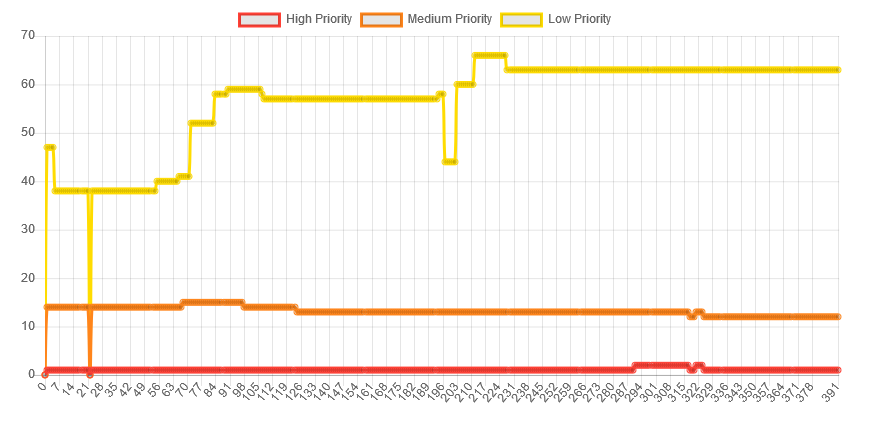
\includegraphics[width=\linewidth]{images/collections_td_timeline.png}
		\caption{Commons Collections}
		\label{fig:collections-td-timeline}
	\end{subfigure}
	\begin{subfigure}{.45\textwidth}
		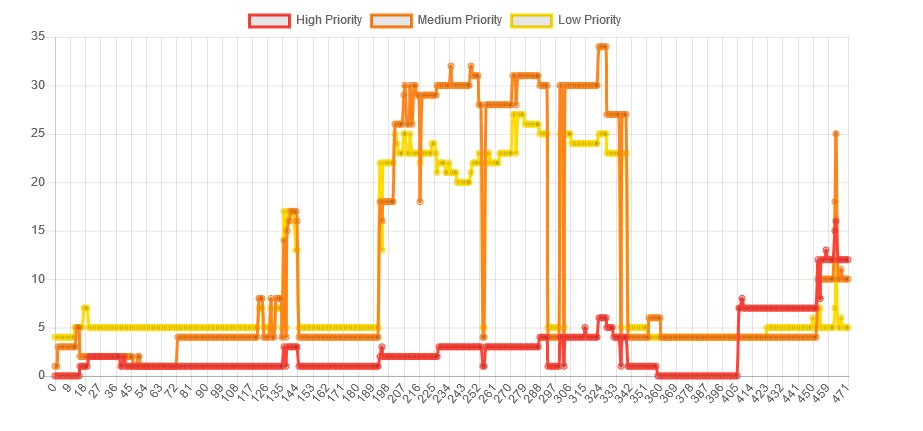
\includegraphics[width=\linewidth]{images/spring_td_timeline.png}
		\caption{Spring HATEOAS}
		\label{fig:spring-td-timeline}
	\end{subfigure}
	\caption{Technical Debt Timeline Comparison}
	\label{fig:td-timeline}
\end{figure*}

The relationship between total technical debt and both work effort calculations
can be seen in figure \ref{fig:td-total-debt}, for the \emph{Checkstyle}
project. Unfortunately, the results do not show any meaningful pattern since
technical debt has remained more or less constant throughout project evolution.
The two subfigures \ref{fig:td-total-debt-commit} and
\ref{fig:td-total-debt-ticket} appear to have a different population count,
possibly due to the difference in the statistics of work effort, mapped on the
\emph{x} axis. For work effort calculated using commit timestamps, the data
points are overlapping when values for effort are in the range $[0-10]$ whereas
data points are spread out over calculations using ticket timestamps. The
results for the other projects show the same constant pattern. 

\begin{figure*}
	\centering
	\begin{subfigure}{.45\textwidth}
		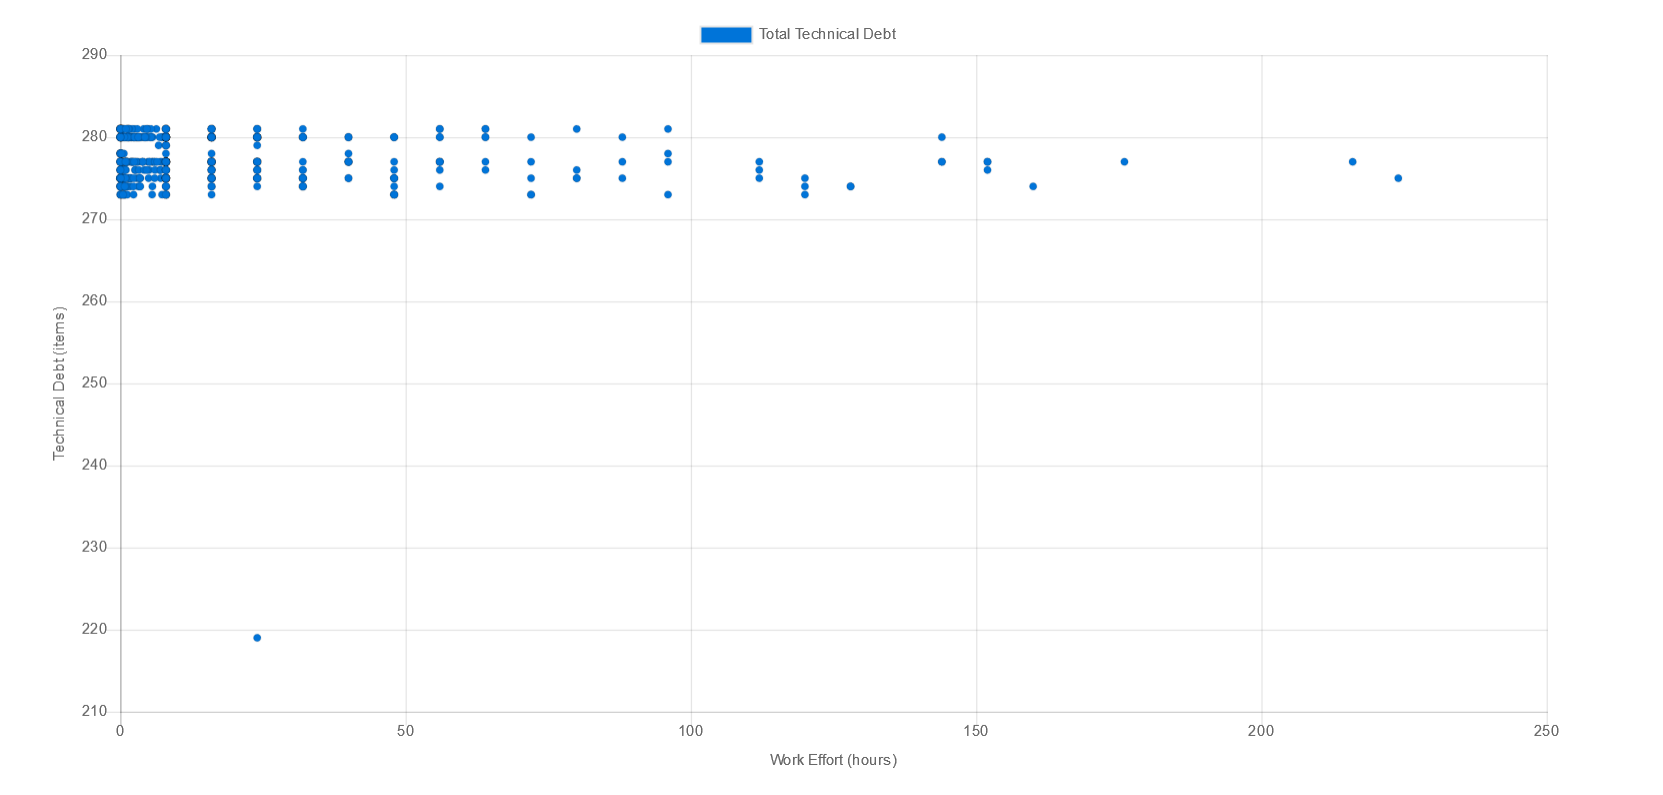
\includegraphics[width=\linewidth]{images/checkstyle_total_debt_commit.png}
		\caption{By Commit Timestamps}
		\label{fig:td-total-debt-commit}
	\end{subfigure}
	\begin{subfigure}{.45\textwidth}
		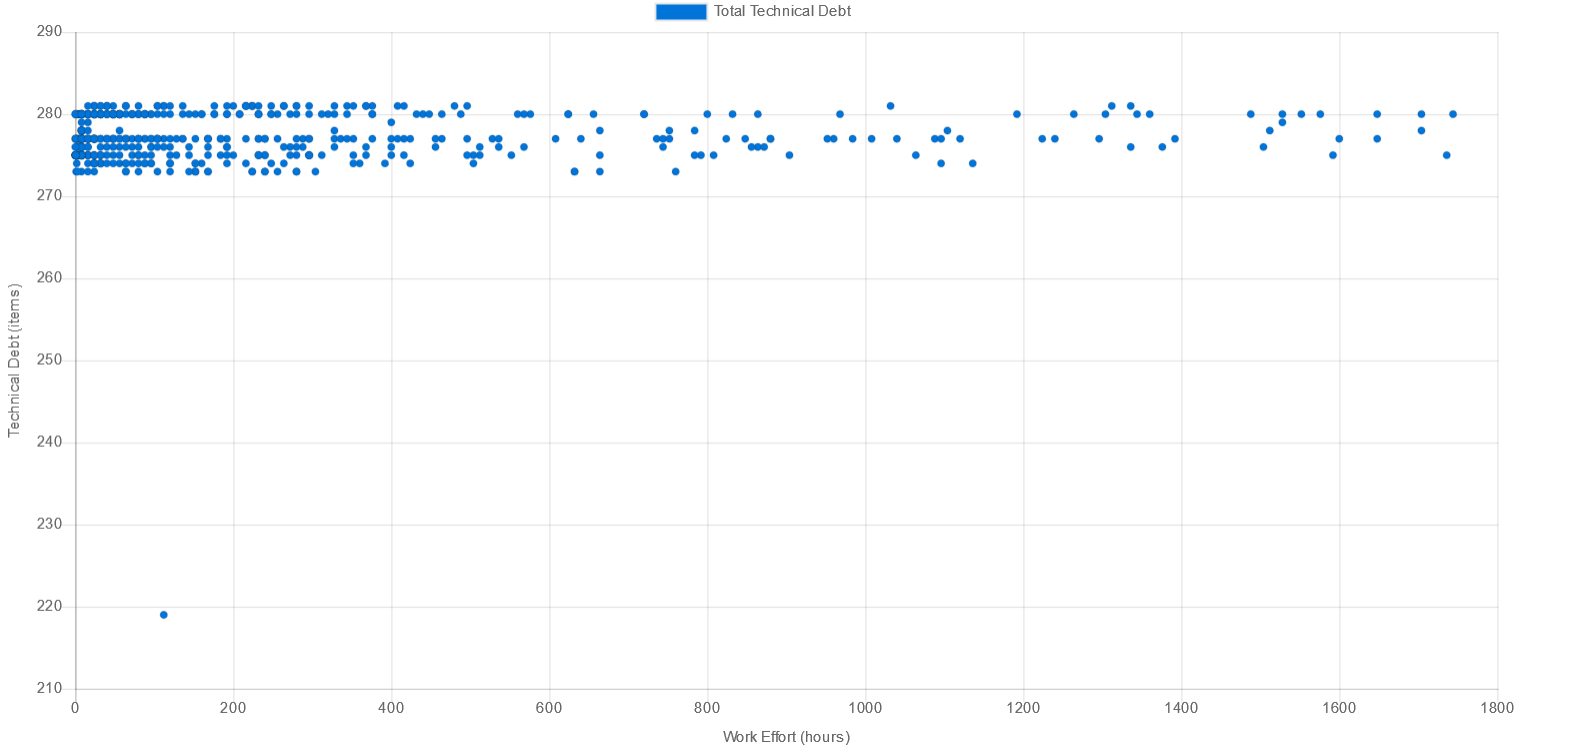
\includegraphics[width=\linewidth]{images/checkstyle_total_debt_ticket.png}
		\caption{By Ticket Timestamps}
		\label{fig:td-total-debt-ticket}
	\end{subfigure}
	\caption{Total Technical Debt and Work Effort for Checkstyle}
	\label{fig:td-total-debt}
\end{figure*}

Since technical debt is constant at the project level, the relationship with
work effort is still unknown. This is most likely due to measuring technical
debt at the project level, which may not affect the productivity at the class
level.

% - - - - - - - - - - - - - - - - - - - - - - - - - - - - - - - - - - - - - - -
\subsubsection*{Experiment 2}
\label{experiment-2}

Since the results of experiment 1 are inconclusive, we applied the
locality-based model for calculating technical debt. As mentioned in section
\ref{data-processing}, the locality model calculates technical debt based on the
change-set of each work task. Only code violations that are in the set of class
changes made by a developer are considered to affect the effort required to
accomplish the task. The statistics can be seen in figure
\ref{tab-technical-debt-local}.

\begin{table*}
	\centering
	\begin{tabular}{ |c|c|r|r|r|r|r| }
		\hline
		\multicolumn{2}{ |c| }{Category}                        & \emph{ANTLR} & \emph{Spring HATEOAS} & \emph{Checkstyle} & \emph{Commons Collections} & \emph{Commons Lang} \\ \hline \hline
		\multicolumn{1}{ |c  }{\multirow{2}{*}{TD Local Pain} } &
		\multicolumn{1}{ |l| }{Mean}                            & 1.814        & 0.34                  & 0.16              & 1.13                       & 6.299               \\ \cline{2-7}
		\multicolumn{1}{ |c  }{}                                &
		\multicolumn{1}{ |l| }{Std}                             & 7.861        & 1.205                 & 0.651             & 3.53                       & 13.635              \\ \cline{1-7}
	\end{tabular}
	\caption{\label{tab-technical-debt-local} Experiment 2: Technical Debt Statistics}
\end{table*}

In contrast to experiment 1, the measurement of technical debt has reduced
dramatically. Although the same population of work items has been used for both
experiments, it seems that for the majority of projects, very few quality issues
on average affect the daily work of a developer. This is surprising, especially
since \emph{ANTLR} had the largest debt per work item out of all candidates. One
factor which might influence the results is the application domain of each
project. A possible explanation for \emph{ANTLR} is that, because the project is
a language generation tool, many files of its source code could be grammar files
which SpotBugs does not analyse. Thus it is possible that many tasks revolve
around changes to these files, and the detected quality issues do not affect
developer productivity. 

\begin{figure*}
	\centering
	\begin{subfigure}{.45\textwidth}
		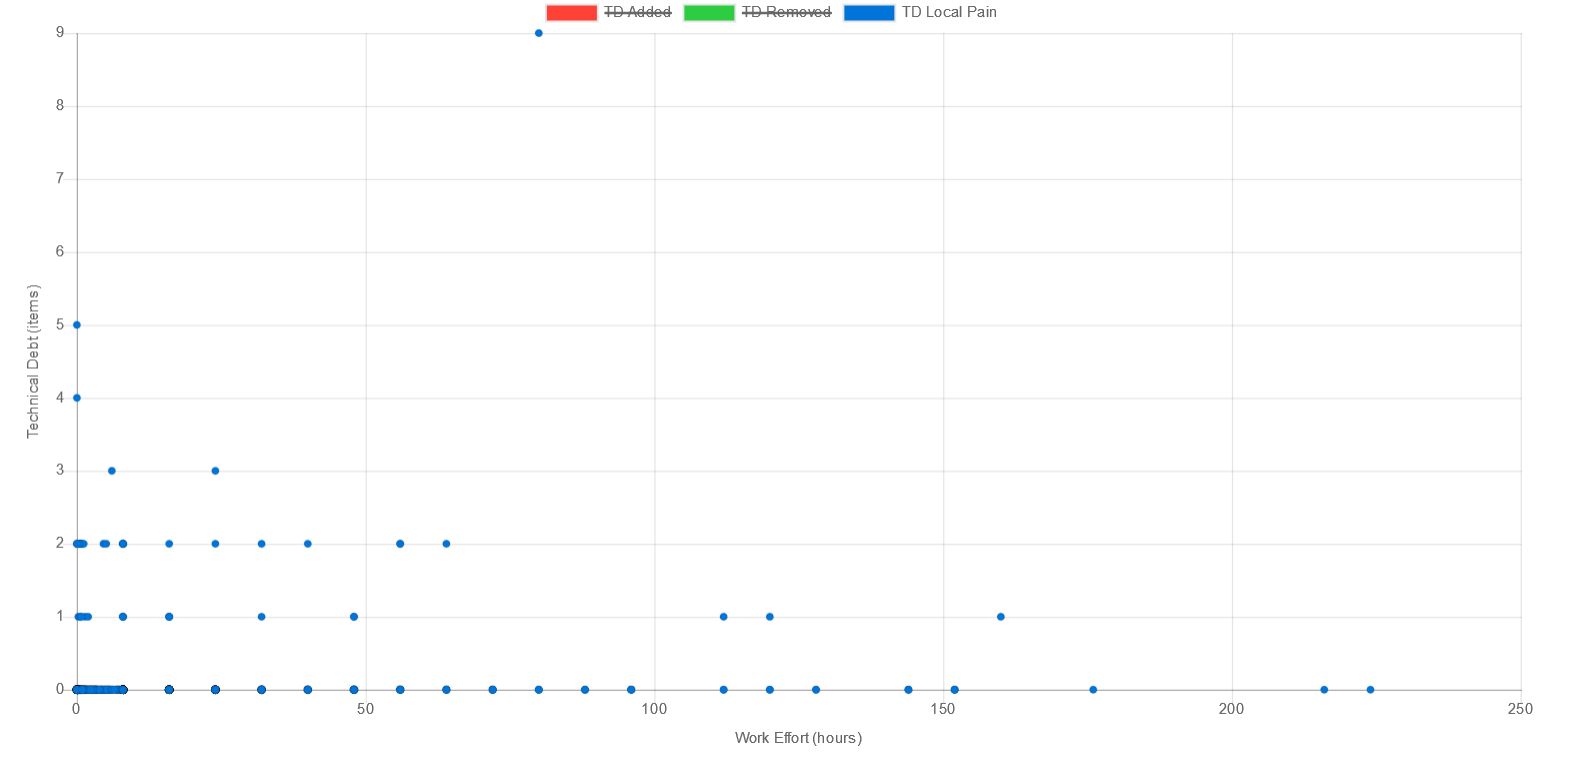
\includegraphics[width=\linewidth]{images/checkstyle_local_debt_commit.png}
		\caption{By Commit Timestamp}
		\label{fig:collections-td-timeline}
	\end{subfigure}
	\begin{subfigure}{.45\textwidth}
		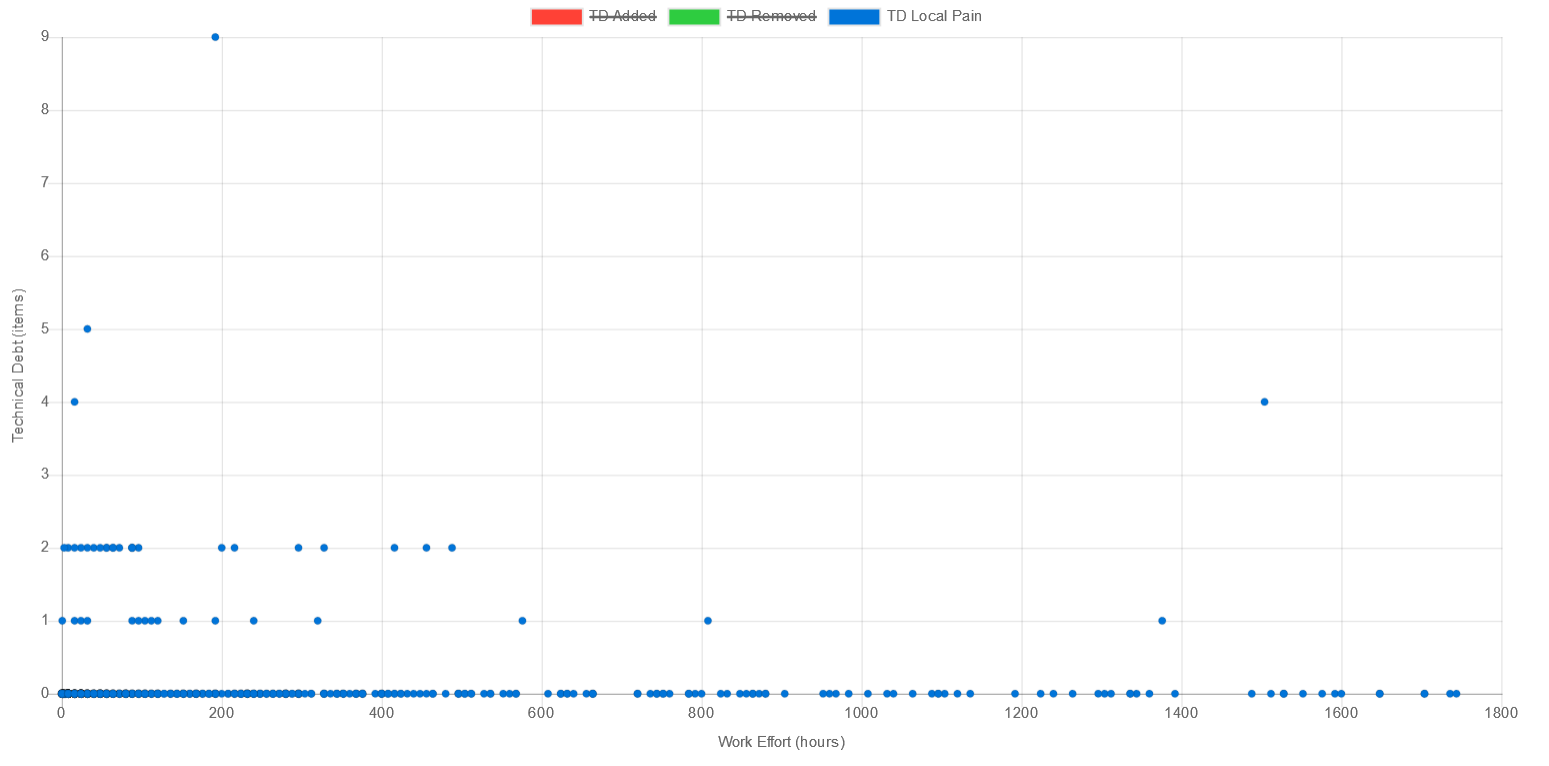
\includegraphics[width=\linewidth]{images/checkstyle_local_debt_ticket.png}
		\caption{By Ticket Timestamp}
		\label{fig:spring-td-timeline}
	\end{subfigure}
	\caption{Local Technical Debt and Work Effort for Checkstyle}
	\label{fig:td-local-debt}
\end{figure*}

The relationship between local technical debt and work effort per task can be
seen in figure \ref{fig:td-local-debt}, for \emph{Checkstyle}. The results seem
to have spread out since technical debt is not as constant due to the change in
``level'' where technical debt items are considered to affect work. Similar to
\ref{fig:td-total-debt}, data points for the commit timestamp method are
concentrated in the range $[0-10]$ hours on the work effort axis due to the
calculations. On the other hand, they are spread out for the ticket method due
to the high variance of work effort previously calculated. The pattern by all
projects is the same. Many data points are unaffected by quality issues found,
and even the number of issues found do not vary as much as expected. One
possibility is that work items include minimal changes to classes that are
unaffected by debt. Another possibility is that types of quality issues found by
the static analysis tools at the code level are not as severe as those at the
architectural level. We propose further research on the topic in section
\ref{future-work}. 

\begin{table*}
	\centering
	\begin{tabular}{ |c|c|r|r|r|r|r| }
		\hline
		\multicolumn{2}{ |c| }{Category}                        & \emph{ANTLR} & \emph{Spring HATEOAS} & \emph{Checkstyle} & \emph{Commons Collections} & \emph{Commons Lang} \\ \hline \hline
		\multicolumn{1}{ |c  }{\multirow{2}{*}{TD Added} }      &
		\multicolumn{1}{ |l| }{Mean}                            & 40.561       & 0.325                 & 4.814             & 3.493                      & 4.918               \\ \cline{2-7}
		\multicolumn{1}{ |c  }{}                                &
		\multicolumn{1}{ |l| }{Std}                             & 168.236      & 1.49                  & 19.525            & 10.196                     & 16.139              \\ \cline{1-7}

		\multicolumn{1}{ |c  }{\multirow{2}{*}{TD Removed} }    &
		\multicolumn{1}{ |l| }{Mean}                            & 50.598       & 1.593                 & 4.966             & 1.768                      & 4.392               \\ \cline{2-7}
		\multicolumn{1}{ |c  }{}                                &
		\multicolumn{1}{ |l| }{Std}                             & 190.364      & 7.432                 & 19.846            & 5.486                      & 14.605              \\ \cline{1-7}
	\end{tabular}
	\caption{\label{tab-technical-debt-intro} Experiment 3: Technical Debt Statistics}
\end{table*}

% - - - - - - - - - - - - - - - - - - - - - - - - - - - - - - - - - - - - - - -
\subsubsection*{Experiment 3}
\label{experiment-3}

Lastly, the scope of the third experiment was to analyse whether introduction or
removal of debt would impact work effort.  The statistics for technical debt
introduced and removed can be seen in table \ref{tab-technical-debt-intro}. 

\begin{figure*}
	\centering
	\begin{subfigure}{.45\textwidth}
		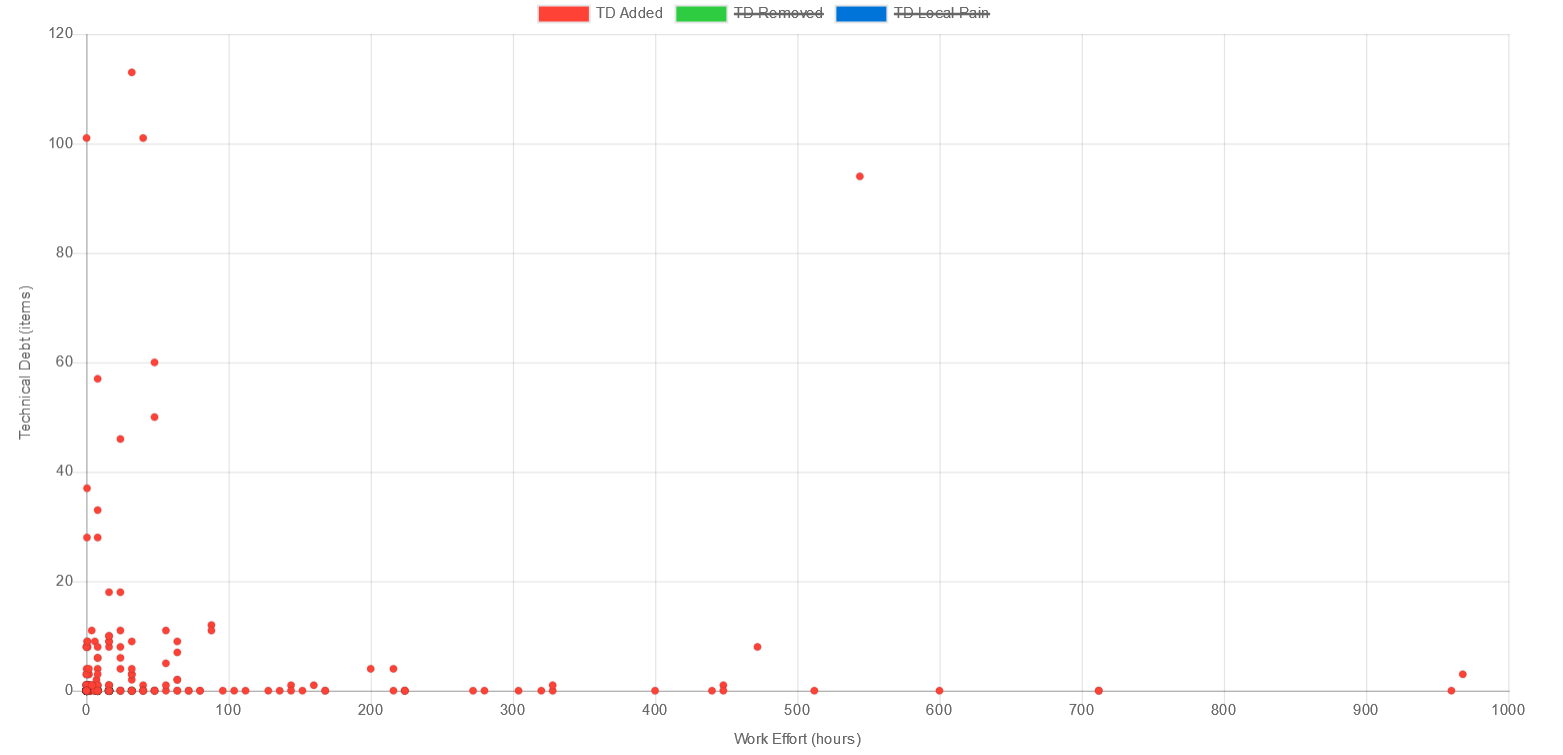
\includegraphics[width=\linewidth]{images/collections_added_debt_commit.png}
		\caption{Total Technical Debt}
		\label{fig:td-added-commit}
	\end{subfigure}
	\begin{subfigure}{.45\textwidth}
		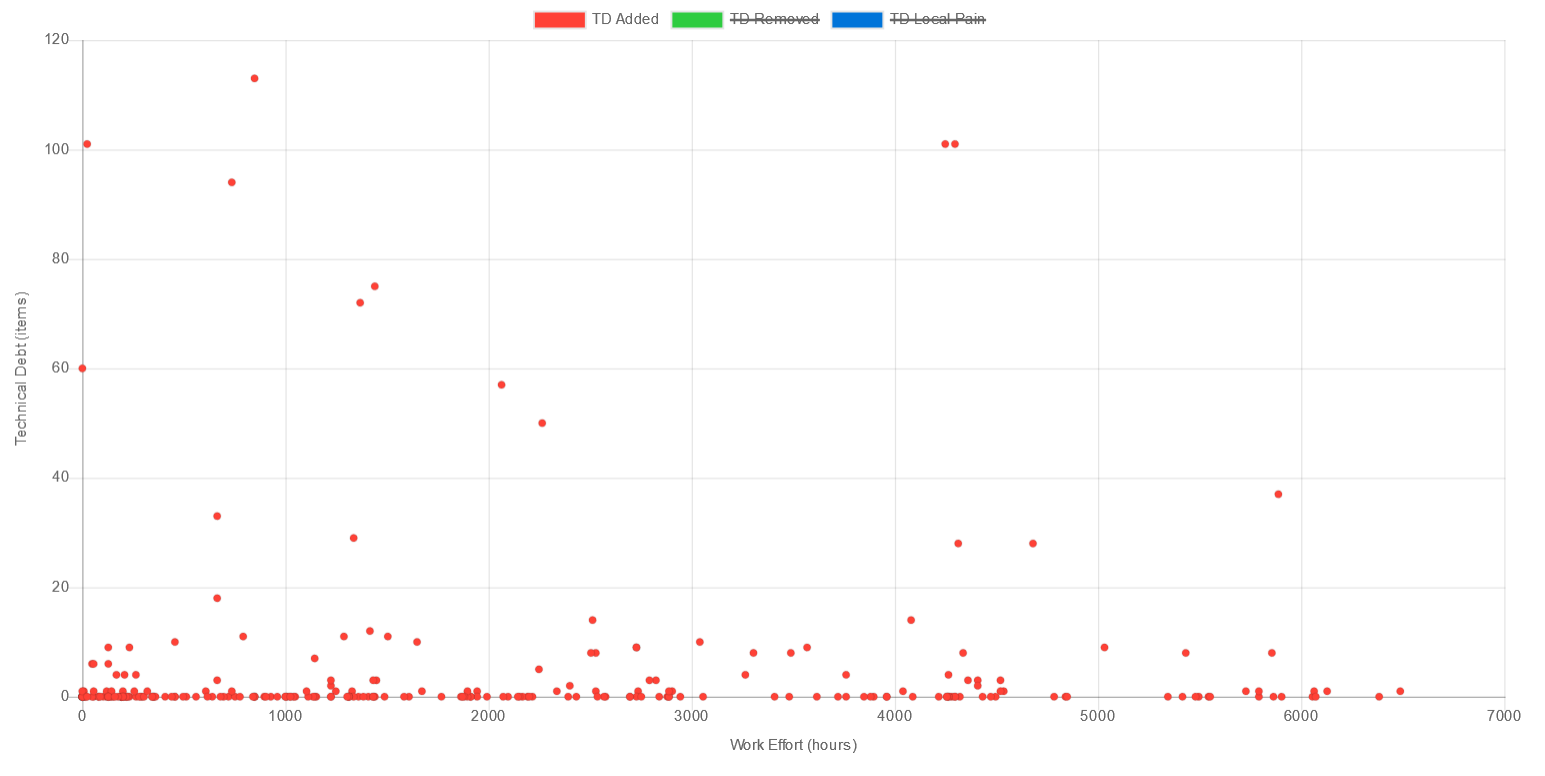
\includegraphics[width=\linewidth]{images/collections_added_debt_ticket.png}
		\caption{Local Technical Debt}
		\label{fig:td-added-ticket}
	\end{subfigure}
	\caption{Technical Debt Added and Work Effort for Collections}
	\label{fig:td-added}
\end{figure*}


It seems that, on average, \emph{ANTLR} has many introductions and removals of
debt items. The developers of \emph{Spring HATEOAS}, since it is a younger
project, are focusing on removal of quality issues to eliminate the threats of
bugs. The other projects have very similar results for both sets of
calculations. It seems that, on average, the number of quality issues introduced
by work items is approximately equal to the number of technical debt items
removed. This might be a consequence of adding new features with initial quality
issues which are refined over time by the team through other tasks such as
fixing bugs and other refactoring activities.

\begin{figure*}
	\centering
	\begin{subfigure}{.45\textwidth}
		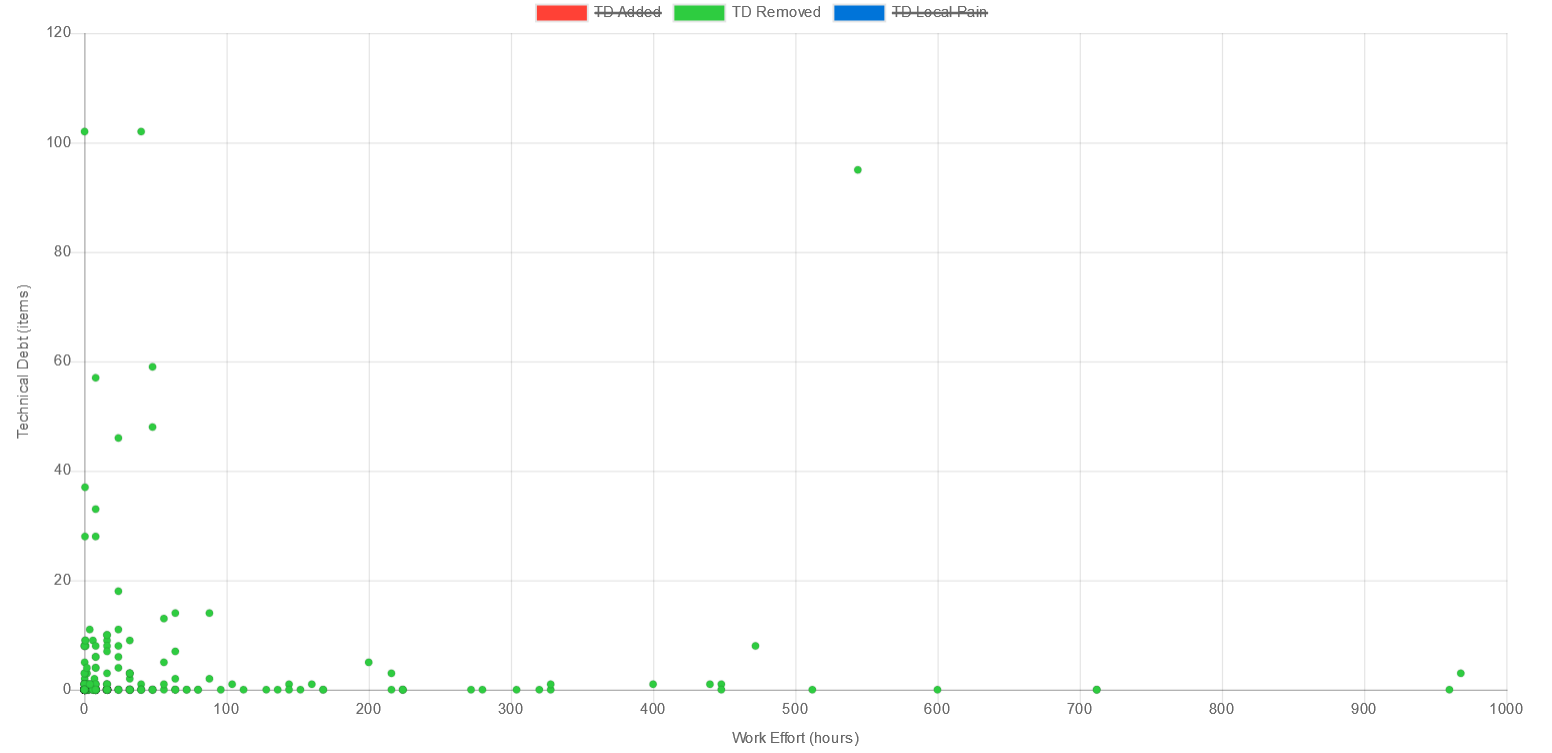
\includegraphics[width=\linewidth]{images/collections_removed_debt_commit.png}
		\caption{By Commit}
		\label{fig:td-removed-commit}
	\end{subfigure}
	\begin{subfigure}{.45\textwidth}
		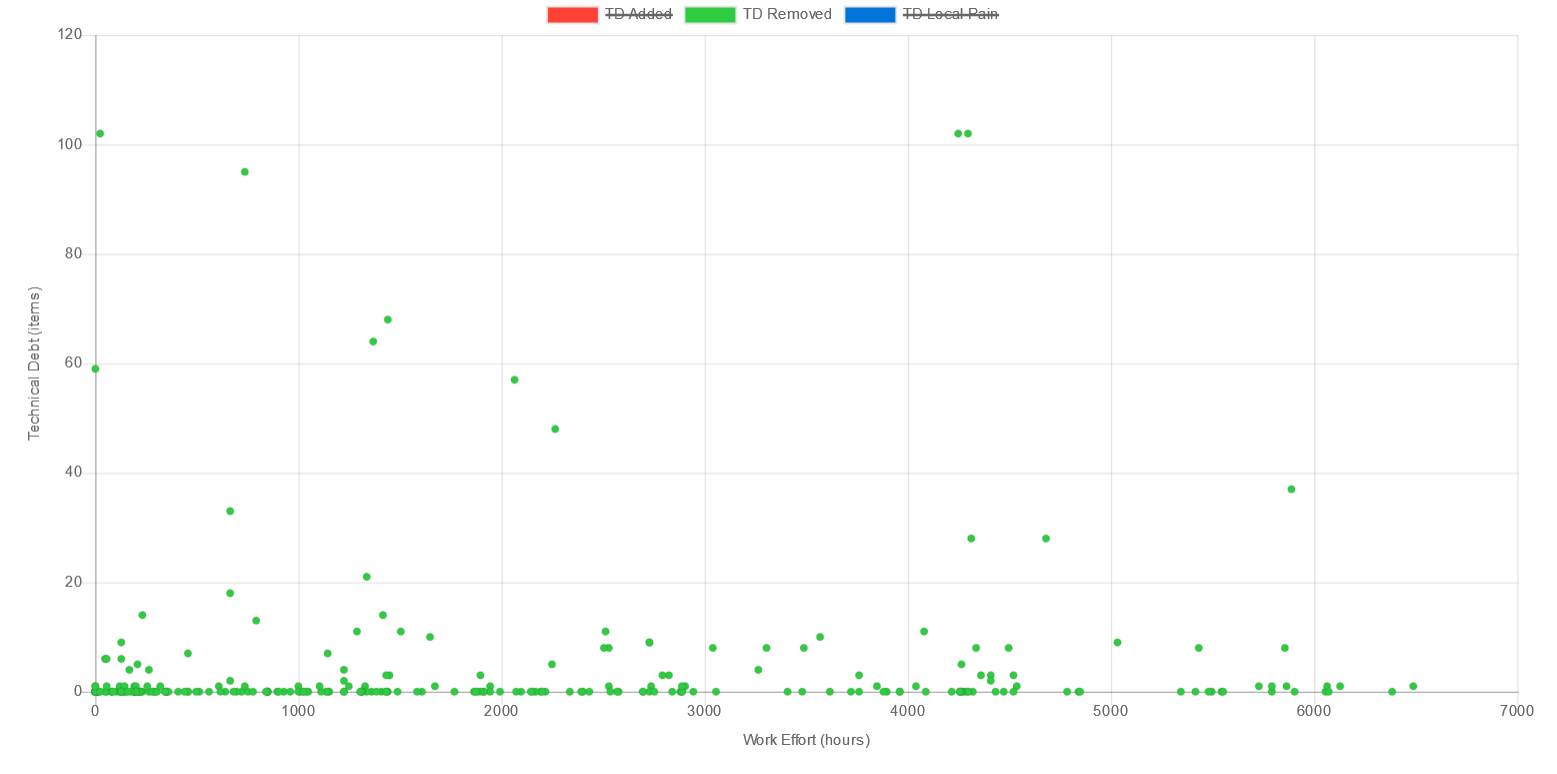
\includegraphics[width=\linewidth]{images/collections_removed_debt_ticket.png}
		\caption{By Ticket}
		\label{fig:td-removed-ticket}
	\end{subfigure}
	\caption{Technical Debt Removed and Work Effort for Collections}
	\label{fig:td-removed}
\end{figure*}

Lastly, the relationship between work effort calculations and technical debt
added and removed are presented in figures \ref{fig:td-added} and
\ref{fig:td-removed}, respectively. The four figures display similar patterns to
the previous local debt relationship with work effort, presented in figure
\ref{fig:td-local-debt}. It seems that as work effort increases, technical debt
decreases. This observation makes sense for removal of technical debt since work
effort should increase with refactoring activities. However, the distribution of
data points is mostly around the range $[0-100]$ hours on the work effort axis.\\


Although the three experiments build on one another, from our perspective, there
is no correlation between work effort and technical debt. The first experiment
showed that technical debt at the project level does affect the effort required
to finish tasks. Additionally, the relationship between work effort and local
technical debt follows a negative pattern, since an increase in work effort
shows a decrease in technical debt. The results of the third experiment share
this pattern as well. We consider the results to be inconclusive due to many
controlled and excluded factors for the simplicity of the calculations.

%%%%%%%%%%%%%%%%%%%%%%%%%%%%%%%%%%%%%%%%%%%%%%%%%%%%%%%%%%%%%%%%%%%%%%%%%%%%%%%
%%%%%%%%%%%%%%%%%%%%%%%%%%%%%%%%%%%%%%%%%%%%%%%%%%%%%%%%%%%%%%%%%%%%%%%%%%%%%%%
%%%%%%%%%%%%%%%%%%%%%%%%%%%%%%%%%%%%%%%%%%%%%%%%%%%%%%%%%%%%%%%%%%%%%%%%%%%%%%%
\section{Validity and Future Work}
\label{validity-future-work}

Throughout the study, there have been numerous simplifying assumptions that may
affect the results and conclusion presented in the earlier section. These range
from each type of calculation to other subjective factors that are difficult to
model in such a short experiment. We consider such factors in this section and
suggest further work for future experiments.

%%%%%%%%%%%%%%%%%%%%%%%%%%%%%%%%%%%%%%%%%%%%%%%%%%%%%%%%%%%%%%%%%%%%%%%%%%%%%%%
\subsection{Threaths to Validity}
\label{validity}

% - - - - - - - - - - - - - - - - - - - - - - - - - - - - - - - - - - - - - - -
\subsubsection*{Work Effort Measurement}
\label{validity-work}

Some simplifying assumptions have been made in the design process of the work
calculation methods. Although such assumptions simplify the method of
computation, it might additionally introduce margins of errors into the results.
The following factors may have had an impact:

\begin{enumerate}
  \item We considered work to have a `linear' pattern. That is, a developer
  works on a single work task at a time and once she finishes the task, work
  starts on the next. This is not always the case since developers may
  collaborate on tasks.

  \item We considered that a developer works on a single item at a time. This
  may not be true. In corporate and open-source environments, it is very likely
  that engineers work on multiple items and/or project at a time.

  \item We did not introduce external workflow variables such as mini breaks for
  coffee, meetings, weekends or time off. This means that work effort results
  may contain non-development time. 

  \item We considered that developers work continously, on 8 hours per day. This
  might not be accurate, especially in open-source projects. Engineers might
  take less time out of their schedule if they are working on a part time basis.

  \item Additionally, we did not consider factors such as technical experience,
  knowledge of the system, familiarity with libraries and dependencies used,
  personality and intrinsic complicated details of the work involved.
  Collecting such data means tracking down and interviewing each project
  collaborator. Moreover, modelling such subjective factors in work effort is a
  complex challenge. 
\end{enumerate}

% - - - - - - - - - - - - - - - - - - - - - - - - - - - - - - - - - - - - - - -
\subsubsection*{Technical Debt Measurement}
\label{validity-td}

Similarly, for technical debt calculations some simplifying assumptions were
introduced to reduce the complexity of measurement:

\begin{enumerate}
  \item The technical debt measurement is a simple count of all quality issues
  found per revision. We did not consider the severity of the quality issues.
  \item The data collection phase only analysed the source code for simple code
  bug patterns, whereas technical debt may also appear at the architectural
  level and testing phases.
 \item There are other types of technical debt which have not been considered
  due to complexity in the modelling of such factors. For example, requirements
  debt takes more effort out of a developer's time to understand the underlying
  task at hand.
\end{enumerate}

Although these assumptions are simplistic, they have been added for this
purpose. Due to the nature of the variables involved, it is challenging to model
specific factors into the computations without supporting data. Therefore, we
hope that this experiment will be the starting point for further research in
this area. 

%%%%%%%%%%%%%%%%%%%%%%%%%%%%%%%%%%%%%%%%%%%%%%%%%%%%%%%%%%%%%%%%%%%%%%%%%%%%%%%
\subsection{Future Work}
\label{future-work}

The results shown require a few changes to the underlying computation methods
for work effort and technical debt accuracy. First of all, future research in
this area should consider a more complex identification mechanism and
computation of technical debt measurement. There is value in identifying quality
issues at the test and architecture level for various modules of projects and
see how these may affect work effort in comparison with code debt. Fontana et
al. \cite{Fontana2016} and Letouzey et. al \cite{Letouzey2012} have devised for
complex calculations for measuring technical debt that could be tailored for the
data collection pipeline mentioned in section \ref{data-collection}.

Gathering more data on the subjective aspect of the team, possibly through
questionnaires and interviews might yield more accurate results for work effort
as well as a convincing validation method. This would command a greater
understanding of development patterns and provide additional data to the
computation and validation of work effort.

Additional experiments may expand on the data collected from the project
management tool. For example, it would be interesting if there is any
correlation between work effort and tickets types such as features, enhacements
and bugs. Moreover, ticket complexity plays a great role in assessing an initial
work effort and would an interesting to note how technical debt affects the
actual work effort in relation to the initial early estimation. Additional
expansions of this experiment would also look at ticket priority and how
technical debt varies between the starting and ending revision of work tasks. 

Furthermore, the relationship between technical debt and change-sets could be
explored in more detail. It would be beneficial to explore whether the number of
changes per files is affected by a local and global measurement of technical
debt. In addition, the change-set size may give an accurate representation of
the work effort involved for delivery of a task. However, this assumption may
backfire as many Integrated Development Environments (IDEs) integrate
refactoring tools which may hinder results. A solution would be to detect and
exclude such refactorings by statically analysing the code \cite{Silva2017}.
Moreover, change-sets may also give an idea of the complexity of the work
involved by measuring the entropy of changes for each revision in relation to
the rest of the code base \footnote{https://github.com/GripQA/commit-entropy}. 

Lastly, it would be beneficial to expand the number of candidates and include a
varied set of domains, languages, version control systems and project management
tools.

%%%%%%%%%%%%%%%%%%%%%%%%%%%%%%%%%%%%%%%%%%%%%%%%%%%%%%%%%%%%%%%%%%%%%%%%%%%%%%%
%%%%%%%%%%%%%%%%%%%%%%%%%%%%%%%%%%%%%%%%%%%%%%%%%%%%%%%%%%%%%%%%%%%%%%%%%%%%%%%
%%%%%%%%%%%%%%%%%%%%%%%%%%%%%%%%%%%%%%%%%%%%%%%%%%%%%%%%%%%%%%%%%%%%%%%%%%%%%%%
\section{Conclusion}
\label{conclusion}

To conclude, technical debt is a phenomenon difficult to measure accurately and
assess potential development and business costs. Therefore, understanding it
from the perspective of developers is vital as they are first-hand involved in
the implementation of new features. Any extra work spent as a result of
previously incurred debt increases business costs. If too much debt accrues over
the lifetime of a project, the entire project may be brought to a stand-still.

Throughout this paper, we presented a method for gathering information from
three fundamental systems of any software engineering environment, how to model
and centralise such data for further processing and analysis. Two methods for
computing work effort have been described: using issue tracking metadata and
version control logs. 

Although the results do not show any correlation between technical debt and work
effort hopefully further expansion of this study will lay down a foundation for
future research in the domain of technical debt and its impact on the
development environment.

%%%%%%%%%%%%%%%%%%%%%%%%%%%%%%%%%%%%%%%%%%%%%%%%%%%%%%%%%%%%%%%%%%%%%%%%%%%%%%%
%%%%%%%%%%%%%%%%%%%%%%%%%%%%%%%%%%%%%%%%%%%%%%%%%%%%%%%%%%%%%%%%%%%%%%%%%%%%%%%
%%%%%%%%%%%%%%%%%%%%%%%%%%%%%%%%%%%%%%%%%%%%%%%%%%%%%%%%%%%%%%%%%%%%%%%%%%%%%%%
{\bf Acknowledgments.} I would like to thank my supervisor, Dr. Tim Storer, for
his guidance, continued support and patience throughout this year. Many thanks
to the University of Glasgow Computing Science Support Team and to our corporate
partners for their technical support. I would also like to thank my parents and
my girlfriend, Ioana, for their continued love, support and encourangement. 

\bibliographystyle{abbrv}
\bibliography{mdiss}

\end{document}